% Responsables: Pasos 1, 2 y teoría del 4: Persona 1. Paso 3: Persona 4.
% Numérico del 4: Persona 2. Paso 5: Persona 3. ~900 palabras en total.
\section{Solución del problema del cliente}

\subsection{Paso 1. Mercator}

La proyección más sencilla es tomar $f(w) = R\,w$, es decir,
\begin{equation}
  x = R\,\lon, \qquad y = R\,q(\lat) = R\ln\tan\!\left(\frac{\pi}{4}+\frac{\lat}{2}\right).
  \label{eq:mercator}
\end{equation}
Esta es la proyección de Mercator. Como $f' = R \neq 0$, es conforme, y por
\eqref{eq:sigma} su factor de escala es
\begin{equation}
  \sigma_{\mathrm{M}}(\lat) = \frac{R}{R\cos\lat} = \sec\lat .
  \label{eq:sigma_mercator}
\end{equation}
En México va de $\sec(14.53^\circ) \approx 1.033$ en la frontera con
Guatemala a $\sec(32.72^\circ) \approx 1.189$ en Baja California: la misma
distancia se ve un 15\,\% más larga en el norte que en el sur, como
sospechaban los analistas del cliente. Además, de $\zeta = R\,e^{iw}$ se
despeja
\begin{equation}
  R\,w = -iR\,\log\!\left(\frac{\zeta}{R}\right),
  \label{eq:mercator_log}
\end{equation}
así que Mercator es, salvo una rotación de $-90^\circ$ y un factor $R$, el
logaritmo complejo de la proyección estereográfica.

\subsection{Paso 2. Cónica Conforme de Lambert}

Ahora tomemos $f(w) = R F e^{inw}$ con constantes $0 < n < 1$ y $F > 0$. Es
analítica con $f' \neq 0$, así que es conforme. En forma polar,
\begin{equation}
  z = \rho\, e^{i n \lon}, \qquad \rho(\lat) = R F e^{-n q(\lat)} :
  \label{eq:lambert_polar}
\end{equation}
los meridianos se vuelven rayos y los paralelos, arcos: $e^{inw}$ enrolla la
franja $-\pi < \lon \le \pi$ en un sector de ángulo $2\pi n$, un cono
desenrollado. Como
$|e^{inw}| = e^{-nq}$, se tiene $|f'| = nRF\,e^{-nq}$ y
\begin{equation}
  \sigma_{\mathrm{L}}(\lat) = \frac{n F e^{-n q(\lat)}}{\cos\lat}, \qquad
  \ln\sigma_{\mathrm{L}} = \ln(nF) - n\,q(\lat) - \ln\cos\lat .
  \label{eq:lambert}
\end{equation}
Pedir escala exacta en dos paralelos estándar, $\sigma(\lat_1) = \sigma(\lat_2)$, da
$-n q(\lat_1) - \ln\cos\lat_1 = -n q(\lat_2) - \ln\cos\lat_2$, de donde
\begin{equation}
  n = \frac{\ln(\cos\lat_1/\cos\lat_2)}{q(\lat_2) - q(\lat_1)},
  \qquad
  F = \frac{\cos\lat_1\, e^{n q(\lat_1)}}{n},
  \label{eq:lambert_n}
\end{equation}
donde $F$ se eligió para que $\sigma(\lat_1) = \sigma(\lat_2) = 1$. Con los
paralelos de INEGI, $\lat_1 = 17.5^\circ$ y $\lat_2 = 29.5^\circ$, resulta
$n \approx 0.3995$.

Entre los dos paralelos la escala es menor que 1. Derivando \eqref{eq:lambert}
con $dq/d\lat = \sec\lat$,
\begin{equation}
  \frac{d\ln\sigma_{\mathrm{L}}}{d\lat} = \frac{\sin\lat - n}{\cos\lat} = 0
  \quad\Longleftrightarrow\quad \sin\lat = n ,
  \label{eq:lambert_min}
\end{equation}
así que el mínimo de $\sigma_{\mathrm{L}}$ está en $\lat = \arcsin n \approx
23.5^\circ$, a la mitad del país.

\subsection{Paso 3. Medir la distorsión}

Para comparar proyecciones se usa la oscilación de $\ln\sigma$ sobre la región,
\begin{equation}
  \dist = \max_{\region} \ln\sigma - \min_{\region} \ln\sigma ,
  \label{eq:delta}
\end{equation}
que no cambia si el mapa se multiplica por una constante: $e^{\delta}$ es el
cociente entre la mayor y la menor escala del mapa. Si se reescala para que
$\sigma$ quede entre $e^{-\delta/2}$ y $e^{\delta/2}$, el error máximo de
escala es $100\,(e^{\delta/2}-1)\,\%$. Evaluando $\sigma$ en una malla de
$0.05^\circ$ dentro del contorno y sobre él:
\begin{itemize}
  \item \textbf{Mercator.} $\ln\sigma = -\ln\cos\lat$ crece con la latitud,
    así que $\sigma$ va de $1.0331$ en el extremo sur a $1.1886$ en el norte y
    $\delta_{\mathrm{M}} = 0.140$. Aun reescalado, el error máximo es de
    $7.3\,\%$; con escala exacta en el ecuador, como en los mapas web, llega
    a $18.9\,\%$.
  \item \textbf{Lambert de INEGI.} Por \eqref{eq:lambert_min}, $\sigma$ baja a
    $0.9945$ en $23.5^\circ$\,N y sube a $1.0077$ en el extremo norte (en el
    extremo sur vale $1.0067$), así que $\delta_{\mathrm{L}} = 0.0132$. El error
    máximo es de $0.66\,\%$ reescalado y de $0.77\,\%$ con la escala de INEGI.
\end{itemize}
Lambert distorsiona unas 10 veces menos que Mercator.

\subsection{Paso 4. Proyección óptima de Chebyshev}
\label{sec:paso4}
\subsubsection*{Planteamiento}

La pregunta es qué función analítica da la menor $\dist$ sobre México.
Tomando logaritmo en \eqref{eq:sigma},
\begin{equation}
  \ln\sigma = h - \ln(R\cos\lat), \qquad h = \ln|f'| ,
  \label{eq:lnsigma}
\end{equation}
donde $h$ es armónica en $\region$ por \eqref{eq:lnfprima}. El segundo término
no depende de la proyección: es el factor de la métrica \eqref{eq:metrica}, y
en él está la curvatura de la esfera. Como $\cos\lat = \operatorname{sech} q$,
se tiene $-\ln(R\cos\lat) = \ln\cosh q - \ln R$, y con $\nabla^2 h = 0$,
\begin{equation}
  \nabla^2_w \ln\sigma = \frac{d^2}{dq^2}\ln\cosh q = \operatorname{sech}^2 q
  = \cos^2\lat > 0 ,
  \label{eq:subarmonica}
\end{equation}
así que $\ln\sigma$ \emph{no} es armónica, sino subarmónica, para cualquier
proyección conforme. Por el principio del máximo, su máximo siempre está en
la frontera $\frontera$.

El teorema de Chebyshev, enunciado en 1856 y demostrado por D.~A. Grave en
1896, dice que la proyección óptima es la que tiene escala constante en la
frontera; aquí seguimos la demostración de Milnor \cite{milnor1969}. Por
\eqref{eq:lnsigma}, pedir $\sigma = e^{c}$ en $\frontera$ es lo mismo que
\begin{equation}
  \nabla^2 h = 0 \text{ en } \region, \qquad
  h = \ln(R\cos\lat) + c \text{ en } \frontera ,
  \label{eq:dirichlet}
\end{equation}
que es un problema de Dirichlet con solución única $h^*$. La constante $c$
solo multiplica el mapa por $e^{c}$ y no cambia $\dist$.

\paragraph{Por qué es óptima.} Sea $\sigma^*$ el factor de la proyección de
Chebyshev. Por \eqref{eq:subarmonica}, el máximo de $\ln\sigma^*$ es $c$ y se
alcanza en $\frontera$; sea $m^*$ su mínimo, alcanzado en un punto $p$, de modo
que $\delta^* = c - m^*$. El punto $p$ es interior: si estuviera en la
frontera, $\ln\sigma^*$ valdría $c$ en todo $\region$, lo que contradice
\eqref{eq:subarmonica}. Cualquier otra proyección conforme tiene
$\ln\sigma = \ln\sigma^* + u$ con $u = h - h^*$ armónica. Si $b \in \frontera$
es donde $u$ alcanza su máximo en la frontera, el principio del máximo da
$u(b) \geq u(p)$, y entonces
\begin{equation}
  \delta \;\geq\; \ln\sigma(b) - \ln\sigma(p)
  = \bigl(c + u(b)\bigr) - \bigl(m^* + u(p)\bigr)
  \;\geq\; c - m^* = \delta^* .
  \label{eq:optimalidad}
\end{equation}
La igualdad exige $u(b) = u(p)$, es decir, que $u$ alcance su máximo en un
punto interior, lo que solo pasa si $u$ es constante. La proyección de
Chebyshev es entonces la única óptima, salvo escala, rotación y traslación
\cite{milnor1969,bermejo2005}.

Para construirla, la conjugada $\tilde h^*$ da $f' = \exp(h^* + i\tilde h^*)$,
y como $\region$ es simplemente conexa, $f = \int f'\,dw$ no depende del
camino.

\subsubsection*{Solución numérica}

El contorno de México continental (2061 vértices) se lleva al plano $w$ con
$w = \lon + i\,q(\lat)$, midiendo $\lon$ desde $102^\circ$\,O. Ahí se
resuelve \eqref{eq:dirichlet} con $c = 0$ por diferencias finitas
(sección~\ref{sec:metodo}) con paso $0.001$ (unos 6~km), en menos de un
segundo. La conjugada sale de integrar $d\tilde h = -h_q\,d\lon + h_\lon\,dq$
sobre la malla, y $f$ de integrar $f' = R\exp(h + c + i\tilde h)$, con $f = 0$
y el norte hacia arriba en $(23.5^\circ$\,N, $102^\circ$\,O$)$ y $c$ elegida
para centrar la escala en 1.

El resultado confirma la teoría: $\ln\sigma \le 0$ en todo el interior
(su máximo es $-9\times10^{-10}$), como exige \eqref{eq:subarmonica}, y su
mínimo está en $24.0^\circ$\,N, $102.3^\circ$\,O. La distorsión de la
proyección óptima es
\begin{equation}
  \delta^* = 0.00184 ,
  \label{eq:delta_optima}
\end{equation}
así que $\sigma$ queda entre $0.99908$ y $1.00092$: un error máximo de escala
de $0.092\,\%$. Su distorsión es 7 veces menor que la de Lambert
($\delta = 0.0132$) y 76 veces menor que la de Mercator ($\delta = 0.140$). El
valor no cambia al refinar la malla ni al simplificar más o menos el contorno
(queda entre $0.001843$ y $0.001844$). En la figura~\ref{fig:sigma}, Mercator y
Lambert cambian por franjas de latitud, mientras que la óptima es mínima en
el centro y sube por igual hacia todo el borde.

\begin{figure}[ht]
  \centering
  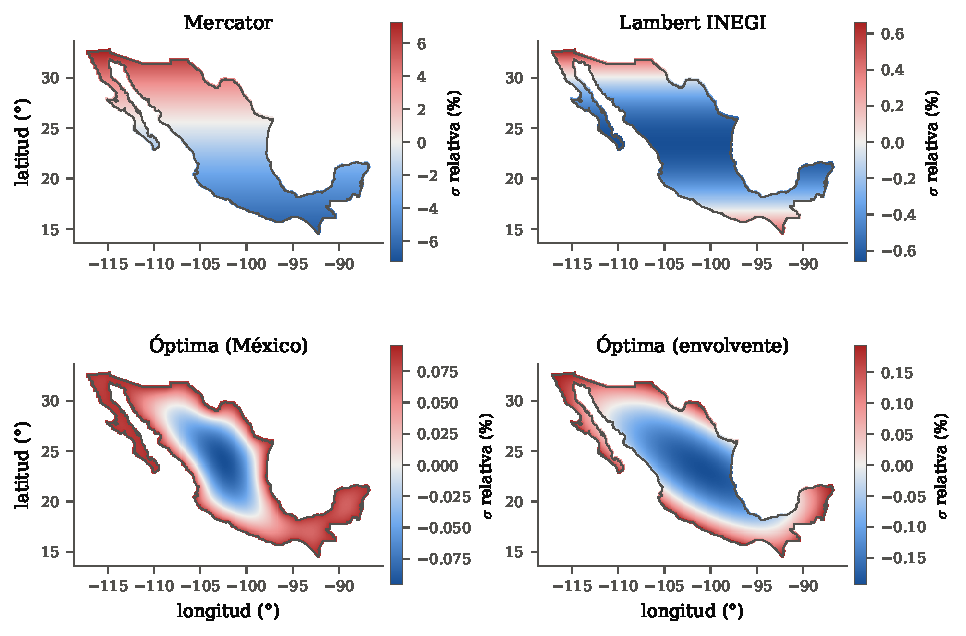
\includegraphics[width=\linewidth]{fig2_sigma}
  \caption{Factor de escala sobre México para cada proyección, reescalado para
    quedar centrado en 1, como desviación en por ciento; la escala de color
    cambia de panel a panel. En la óptima sobre México $\sigma$ es
    prácticamente constante en todo el borde (condición de Chebyshev); en la de
    la envolvente lo es sobre la envolvente convexa. Fuente: elaboración propia.}
  \label{fig:sigma}
\end{figure}

\subsection{Paso 5. Efecto en los datos del cliente}

\paragraph{Datos.} La región $\region$ es México continental, sin islas: la
unión de las 32 entidades del Marco Geoestadístico del INEGI
\cite{inegi_catalogo}, simplificada a 1~km (2061 vértices). Como datos se usan
las cabeceras de los 2478 municipios, tomadas del Catálogo Único de Claves
Geoestadísticas del INEGI (consultado el 26 de noviembre de 2026; en las
alcaldías de la Ciudad de México, la localidad sede). Sin las dos que están en
islas quedan 2476 puntos, que se asignan por entidad a tres regiones: Norte
(BC, BCS, Son., Chih., Coah., NL, Tamps., Dgo., Sin., Zac.; 400 puntos), Sur
(Camp., Chis., Gro., Oax., Q.\,Roo, Tab., Ver., Yuc.; 1136) y Centro (el
resto; 940).

\paragraph{Distancias.} Se tomaron 20\,000 pares al azar dentro de cada región
y 20\,000 en todo el país, y se comparó la distancia euclidiana en cada
proyección con la haversine (figura~\ref{fig:errores}). Con Mercator la mediana
del error es de $5.0\,\%$ en el Sur, $6.3\,\%$ en el Centro y $11.6\,\%$ en el
Norte, con máximos de $18.6\,\%$; corregir con una escala constante no basta,
porque en el Norte la mediana sigue en $5.2\,\%$. Con
Lambert la mediana va de $0.12\,\%$ a $0.41\,\%$ según la región y el máximo
es $0.73\,\%$. Con la óptima la mediana baja a $0.02$--$0.06\,\%$, y en los
pares cuyo arco de círculo máximo queda dentro del territorio (el $88\,\%$ de
la muestra) el error nunca pasa de $0.092\,\%$, que es exactamente la cota
$e^{\delta^*/2} - 1$.

La excepción son los pares que cruzan el mar: entre Baja California Sur y
Sinaloa el error de la óptima llega a $1.8\,\%$, porque la cota solo vale
dentro de $\region$. Resolviendo el problema sobre la envolvente convexa de
México, que incluye los dos golfos, $\delta$ sube a $0.0039$, pero el error
máximo en \emph{todos} los pares de la muestra es de $0.19\,\%$.

\paragraph{Agrupamiento y vecinos.} Se corrió k-means ($k = 10$, $20$ y $50$,
diez semillas) desde los mismos centros que un k-means sobre la esfera y se
contaron los puntos que cambian de grupo (emparejando grupos con el método
húngaro). La mediana de cambios es de $0.7$--$1.5\,\%$ con Mercator,
$0.02$--$0.24\,\%$ con Lambert y $0$--$0.02\,\%$ con la óptima; además, en 7 de
30 corridas con Mercator y en una con Lambert más del $5\,\%$ de los puntos
cambió de grupo porque k-means cayó en otra solución. El conjunto de los 10
vecinos más cercanos cambia en el $0.69\,\%$ de los puntos con Mercator, el
$0.08\,\%$ con Lambert y el $0.12\,\%$ con la óptima (dos cabeceras de Baja
California Sur con vecinos al otro lado del golfo).

\paragraph{Áreas.} Las áreas se multiplican por $\sigma^2$. En las cabeceras,
con Mercator ese factor va de $1.07$ en el Sur a $1.41$ en el Norte, así que un
mapa de densidad subestima la del norte hasta en un $24\,\%$ frente al sur. Con Lambert el
factor está entre $0.989$ y $1.015$, y con la óptima entre $0.998$ y $1.002$.

\begin{figure}[ht]
  \centering
  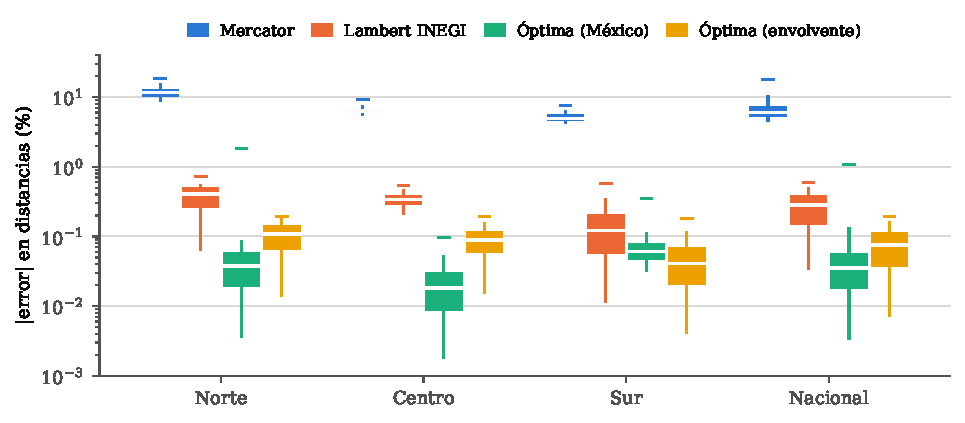
\includegraphics[width=\linewidth]{fig3_errores}
  \caption{Error relativo en distancias entre pares de cabeceras, por región
    y proyección, en escala logarítmica. La caja va del percentil 25 al 75, la
    línea blanca es la mediana, los bigotes van del percentil 5 al 95 y la marca
    aislada es el máximo. Fuente: elaboración propia con datos del INEGI.}
  \label{fig:errores}
\end{figure}
